% A Simple, Extensible Queue Migration Plan for Honcho — M4 deliverable.
% Build:  tectonic one-pager.tex   (figures via one-pager/figures.py first)
\documentclass[10pt]{article}

\usepackage[letterpaper,margin=0.55in,top=0.5in,bottom=0.45in]{geometry}
\usepackage{newpxtext}            % Palatino-like serif — research-note register
\usepackage[T1]{fontenc}
\usepackage{microtype}
\usepackage{graphicx}
\usepackage{multicol}
\usepackage{xcolor}
\usepackage{titlesec}
\usepackage{listings}
\usepackage[hidelinks]{hyperref}

\definecolor{ink}{HTML}{1C2330}
\definecolor{pg}{HTML}{2F6F9F}
\definecolor{valkey}{HTML}{D1495B}
\definecolor{accent}{HTML}{E08A1E}
\definecolor{rule}{HTML}{C3CAD3}
\definecolor{codebg}{HTML}{F4F6F8}

\color{ink}
\setlength{\parindent}{0pt}
\setlength{\parskip}{1.8pt}
\setlength{\columnsep}{18pt}

\titleformat{\section}{\bfseries\large\color{ink}}{}{0pt}{}
\titlespacing{\section}{0pt}{3pt}{1pt}

\lstset{
  basicstyle=\ttfamily\scriptsize\color{ink},
  backgroundcolor=\color{codebg},
  frame=none, breaklines=true, columns=fullflexible,
  keepspaces=true, xleftmargin=4pt, xrightmargin=4pt,
  aboveskip=3pt, belowskip=3pt,
  commentstyle=\color{pg!70!ink}\itshape,
}

\newcommand{\hd}[1]{{\footnotesize\bfseries\color{valkey}#1}\par}

\begin{document}
\thispagestyle{empty}

% ---- masthead -------------------------------------------------------------
{\Large\bfseries A Simple, Extensible Queue Migration Plan for Honcho}\\[2pt]
{\footnotesize\color{ink!70}
Phil Bascom \,$\cdot$\, philbas.com \,$\cdot$\, Platform Engineering take-home
\,$\cdot$\, 2026-06-27 \,$\cdot$\,
\texttt{github.com/philosaether/pl-takehome-technical}}
\vspace{2pt}
{\color{rule}\hrule height 1.2pt}
\vspace{4pt}

% ---- lead / abstract (full width) -----------------------------------------
{\small
This year, the Honcho application saw an orders-of-magnitude explosion in use,
from \mbox{$\sim$200} active users to \mbox{$\sim$30,000}. While its existing
architecture has held up admirably, operational maturity will
require a deliberate choice of implementation methodology.

In this paper, we propose a simple migration plan, with an optional second stage,
and discuss circumstances in which the further migration is advisable. The first
stage requires a minimal, \mbox{$\sim$150-line} alteration to the existing Postgres
queue code, with no new infrastructure. We expect this change to yield a \mbox{$\sim$1000$\times$}
faster scheduling look-ahead, sufficient to support another orders-of-magnitude growth cycle.

The second stage would move some or all work to a Valkey-backed in-memory queue.
While it increases operational complexity and the risk of data loss, we show that
Valkey offers up to 15$\times$ the throughput of Postgres under certain conditions.
}
\vspace{2pt}
{\color{rule}\hrule height 0.4pt}

\begin{multicols}{2}

% ---- §1 -------------------------------------------------------------------
\section*{\small 1\quad Low-hanging fruit is the most nutritious}
{\small
By design, the Honcho deriver processes representation work units only once they
have crossed a threshold of pending cost. Today that value is recomputed every
second by summing message token counts across the queue, grouped by work unit ---
an $O(N)$ scan that grows with queue depth, reaching \mbox{$\sim$2.5\,s} at
$10^{7}$ pending tasks (Fig.~1).

The remedy is to stop recomputing the answer and start maintaining it. We keep
each work unit's pending cost in a small aggregate table, updated incrementally
on enqueue and acknowledgement, and gate eligibility with a partial index the
claim query reads directly. The scan becomes bounded by the number of
\emph{eligible} work units --- a flat, small cost from $10^{4}$ to $10^{7}$
pending tasks. The change is bounded, surgical, and shippable in days (Fig.~2).
}

\begin{center}
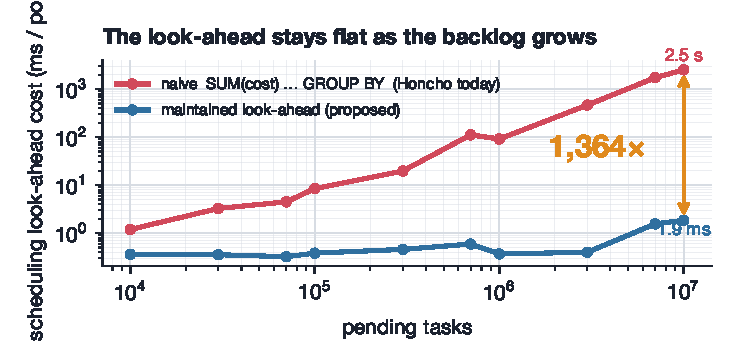
\includegraphics[width=\linewidth]{figures/fig1_lookahead.pdf}
{\scriptsize\color{ink!70}\textbf{Fig.~1.} The maintained look-ahead stays
$\sim$1\,ms; the naive scan reaches 2.5\,s at $10^{7}$ tasks --- a 1{,}364$\times$
gap.\par}
\end{center}

{\scriptsize\textbf{Fig.~2 — the change, against Honcho's real code}
(\texttt{queue\_manager.py\#L347--361}):}
\begin{lstlisting}
# NOW: O(unprocessed tasks), recomputed every poll
select(QueueItem.work_unit_key,
       func.sum(Message.token_count))
  .join(Message).where(~QueueItem.processed)
  .group_by(QueueItem.work_unit_key)   # scan+join
\end{lstlisting}
\begin{lstlisting}
# PROPOSED: O(eligible units), one indexed lookup
select(WorkUnit.work_unit_key)
  .where(WorkUnit.eligible)            # partial index
  .order_by(WorkUnit.oldest_pending_at)
  .with_for_update(skip_locked=True)
\end{lstlisting}

% ---- §2 -------------------------------------------------------------------
\section*{\small 2\quad Efficiency is (sometimes) worth the effort}
{\small
While Postgres-as-queue is a durable pattern --- committed work survives a crash
via write-ahead logging at the OS layer --- Postgres is optimised for
transactional integrity, not raw throughput. A dedicated hot-queue system such as
Valkey offers significantly higher performance under load. That performance comes
at a cost: greater operational complexity, and a risk of data loss through the
fsync window.

Whether Honcho should adopt a Valkey queue is a nuanced question. When tasks are
light-weight and workers execute quickly, Valkey offers a 15$\times$ throughput
increase per primary, and as much as 26$\times$ at equal shard counts under peak
load. But Valkey's lead shrinks to near-parity ($\sim$1.1$\times$) as per-task
time-to-process reaches 200\,ms (Fig.~3).

We advise holding a Valkey migration until production data justifies it. To
support the possibility, average time-to-process and peak worker count should
be tracked as soon as possible.
}

\begin{center}
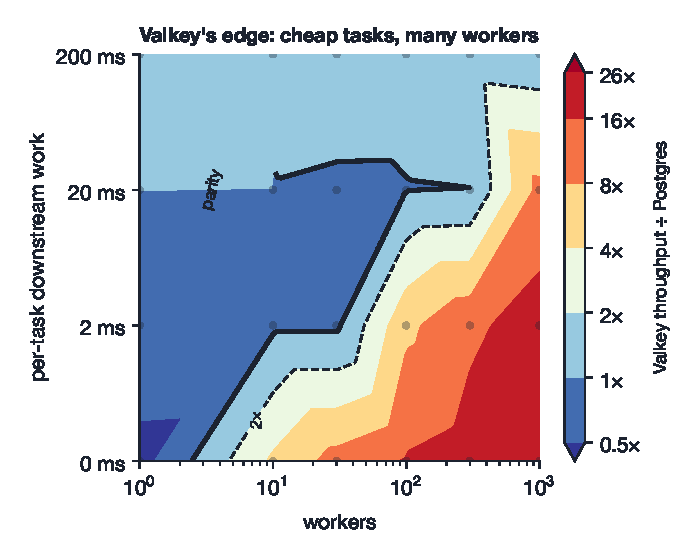
\includegraphics[width=\linewidth]{figures/fig3_manifold_2d.pdf}
{\scriptsize\color{ink!70}\textbf{Fig.~3.} Valkey's throughput advantage over
Postgres across worker count and per-task work. The edge is a canyon for cheap,
high-concurrency work and collapses to parity at LLM-scale latency.\par}
\end{center}

% ---- §3 -------------------------------------------------------------------
\section*{\small 3\quad Methods}
{\small
The look-ahead test ran two near-identical queues differing only in a single SQL
query, isolating the variance to algorithmic complexity, locally in a Docker
container on a 2.6\,GHz MacBook Pro (reproduce under \texttt{tests/bench}).
The head-to-head ran two per-backend Docker images implementing one shared queue
contract against a common load generator on AWS (\texttt{deploy/terraform}); a
Zipfian key distribution drove continuous work-unit churn, and correctness was
established deterministically by the shared \texttt{tests/conformance} package.
Figure~3 interpolates four per-task work levels \{0, 2, 20, 200\,ms\} across
worker counts from 1 to 1{,}000; producer-bound Postgres points are conservative
lower bounds. The full experiment ran in $\sim$90 minutes for under \$10.
}

\end{multicols}

\vspace{1pt}
{\color{rule}\hrule height 0.4pt}
\vspace{2pt}
{\scriptsize\color{ink!85}
\textbf{Reproducibility:} \texttt{make load-test} reproduces the numbers; environment
pinned. \textbf{Fairness:} a per-tenant in-flight cap plus weighted claim order
is the one-seam extension (designed, not built). \textbf{Flush policy:} a per-head age
cap --- every task is promoted when it becomes the oldest and ages out, so one slow task
cannot strand the work behind it. \textbf{Valkey runs on less iron:}
each Valkey primary ran on the \emph{same} box class as Postgres though,
single-threaded, it cannot use it --- so the gap is a conservative floor.
\textbf{Stage-2 hardening:} a standalone reaper, versioned migrations, a managed
durable Valkey tier. \textbf{Sharpening Fig.~3:} 5/50/100\,ms work-points and the
durability curve would resolve the crossover precisely.
}

\end{document}
